% !TEX TS-program = pdflatex
% !TEX encoding = UTF-8 Unicode

% This is a simple template for a LaTeX document using the "article" class.
% See "book", "report", "letter" for other types of document.

\documentclass[11pt]{article} % use larger type; default would be 10pt

\usepackage[utf8]{inputenc} % set input encoding (not needed with XeLaTeX)
\usepackage[english,swedish]{babel}
%%% Examples of Article customizations
% These packages are optional, depending whether you want the features they provide.
% See the LaTeX Companion or other references for full information.

%%% PAGE DIMENSIONS
\usepackage{geometry} % to change the page dimensions
\geometry{a4paper} % or letterpaper (US) or a5paper or....
% \geometry{margin=2in} % for example, change the margins to 2 inches all round
% \geometry{landscape} % set up the page for landscape
%   read geometry.pdf for detailed page layout information

\usepackage{graphicx} % support the \includegraphics command and options
\usepackage{datetime}
\usepackage{amssymb,amsmath} % For mathematical expressions  (Tillagd av Nai) 
\usepackage{textcomp} % For degree sign (Tillagd av Nai) 

%%% NEW COMMANDS
\renewcommand{\dateseparator}{-}
\newdateformat{mydate}{\THEYEAR \dateseparator0\THEMONTH \dateseparator \THEDAY} 
\renewcommand{\figurename}{Figur}

% \usepackage[parfill]{parskip} % Activate to begin paragraphs with an empty line rather than an indent

%%% PACKAGES
\usepackage{booktabs} % for much better looking tables
\usepackage{array} % for better arrays (eg matrices) in maths
\usepackage{paralist} % very flexible & customisable lists (eg. enumerate/itemize, etc.)
\usepackage{verbatim} % adds environment for commenting out blocks of text & for better verbatim
\usepackage{subfig} % make it possible to include more than one captioned figure/table in a single float
% These packages are all incorporated in the memoir class to one degree or another...

%%% HEADERS & FOOTERS
\usepackage{fancyhdr} % This should be set AFTER setting up the page geometry
\pagestyle{fancy} % options: empty , plain , fancy
\renewcommand{\headrulewidth}{0pt} % customise the layout...
\lhead{}\chead{}\rhead{}
\lfoot{}\cfoot{\thepage}\rfoot{}

%%% SECTION TITLE APPEARANCE
\usepackage{sectsty}
\allsectionsfont{\sffamily\mdseries\upshape} % (See the fntguide.pdf for font help)
% (This matches ConTeXt defaults)

%%% ToC (table of contents) APPEARANCE
\usepackage[nottoc,notlof,notlot]{tocbibind} % Put the bibliography in the ToC
\usepackage[titles,subfigure]{tocloft} % Alter the style of the Table of Contents
\renewcommand{\cftsecfont}{\rmfamily\mdseries\upshape}
\renewcommand{\cftsecpagefont}{\rmfamily\mdseries\upshape} % No bold!

%%% END Article customizations






%%% The "real" document content comes below...

\pagenumbering{gobble}
\title{Projektrapport Grupp 3 \\* 
Curling\\*
TNM085 Modelleringsprojekt}
\author{Linnéa Mellblom\\*Linnea Malcherek\\* Julia Nilsson\\*Michael Nilsson\\*Linnéa Nåbo}
%\date{} % Activate to display a given date or no date (if empty),
         % otherwise the current date is printed 
\mydate


\begin{document}
\maketitle
\pagebreak
\pagenumbering{arabic}  

\pagebreak
\tableofcontents
\pagebreak

\section{Introduktion}
Curling är ett intressant system att modellera eftersom det innefattar många vedertagna fysikaliska egenskaper men även delar som inte är särskilt triviala. 
De senaste åren har ett flertal vetenskapliga artiklar publicerats som ger sin förklaring till svängningsfenomenet, den så kallade "curlen" hos curlingstenen.
Gemensamt för artiklarna är hypotesen om att svängningen på curlingstenen beror på en högre friktion bak på stenen än den fram. 
Förklaringen till varför detta är så, har uppdagats det senaste året.. bla bla bla

\subsection{Begränsningar och förenklingar} 
 Denna rapport behandlar modellbygge och simulering av en curlingstens translation och rotation, friktionens påverkan samt kollision mellan curlingstenar. 
Curlingstenarna i beräkningarna har samma massa och därmed kan beräkningar förenklas genom att förkortta bort massan. 
I spelet använder man sig även av sopning för att påverka stenens bana över isen, detta behandlas endast ytligt i denna rapport. 

\section{Fysikalisk beskrivning} 

\subsection{Translation}

I beräkningarna av stenens rörelse har hänsyn tagits till tre påverkande friktionskrafter (Figur~\ref{fig:Translation}): Kraft i riktning motsatt stenens rörelseriktning, samt två krafter i ortogonal riktning mot denna \eqref{Ftot}. Dessa två krafter utgörs av friktionskrafterna i främre delen av stenen samt i den bakre delen. Differensen mellan dessa två krafter är vad som påverkar stenens curl (svängning). 

\begin{subequations}\label{Ftot}
 \begin{align}
 \bar{F_t}&=\bar{F_f}+\bar{F_b}+\bar{F}\\
 \bar{F_f}&<\bar{F_b}
 \end{align}
 \end{subequations}

\begin{figure}[ht!]
\centering
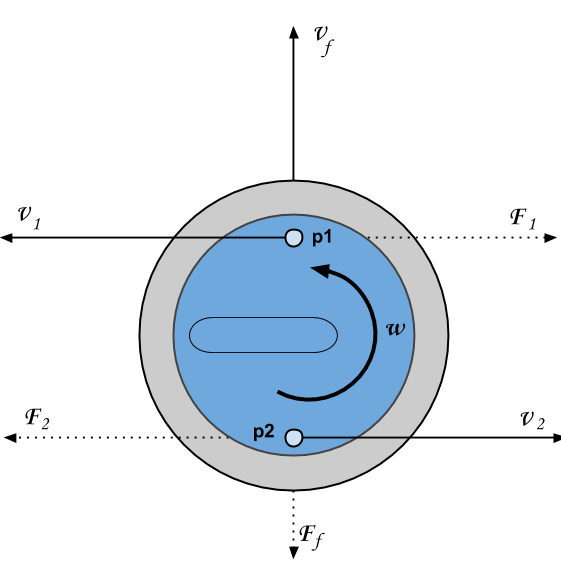
\includegraphics[width=80mm]{Translation.png}
\caption{Påverkan av stenens translation}
\label{fig:Translation}
\label{overflow}
\end{figure}

\subsubsection{Friktionens påverkan}
I kontaktytan mellan isen och curlingstenen uppstår friktion. 
Friktionens påverkan avgörs av stenens kontaktyta samt isens egenskaper. 
Isen påverkas i sin tur av temperatur och luftfuktighet. 
Före spel prepareras isen genom såkallad pebbling då vattendroppar sprids ut över isen och skapar en mindre glatt struktur.
Vid sopning värms isen upp och en tunn vattenhinna skapas framför stenen. Detta gör så att friktion mellan sten och is minskar och därmed går stenen längre vid sopning.  
\\\\Stenens curl beror på att friktionen i den bakre delen \eqref{Fsida2} av stenen är högre än i den främre \eqref{Fsida1}.  
En curlingsten har en kontaktyta mot isen bestående av ett tunt band (ca 5mm brett) som har en något ojämn yta, så kallad scratchad yta. 
När den främre halvan av stenen rör sig över den pebblade isen orsakas ett spår i isen i stenens rörelseriktning med en liten vinkel i rotationsriktningen. 
Då den bakre delen av bandet passerar samma yta ska bandets scratchade yta passera dessa spår, vilka då ligger i nästan rätvinklig riktning från bandets färdriktning, (Figur~\ref{fig:Friktion}). 
Det innebär att den bakre delen av stenen får ett högre motstånd, en högre friktionskraft, än den främre \eqref{biggerthan}. 
REFERENS: http://www.sciencedirect.com/science/article/pii/S0043164813000732

 \begin{align}\label{Fsida1}
 F_1& = ma_1 = \mu_1 mg \Rightarrow a_1 = \mu_1 g \\\label{Fsida2}
 F_2& = ma_2 = \mu_2 mg \Rightarrow a_2 = \mu_2g \\\label{biggerthan}
 \mu_2& > \mu_1
 \end{align}

\begin{figure}[ht!]
\centering
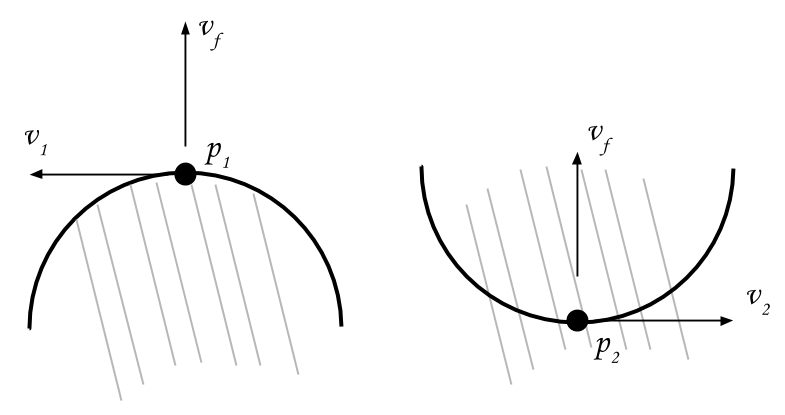
\includegraphics[width=110mm]{Friktion_bakfram.png}
\caption{Friktion i punkt bak respektive fram på stenen. Den bakre delen måste passera de spår framsidan av stenen skapat, vilket leder till högre friktion.}
\label{fig:Friktion}
\label{overflow}
\end{figure}

Den vattenhinna som skapas vid sopning för med sig att de spår som den främre delen av stenen åstadkommer minskar och därmed  även dess effekt på den bakre delen av stenen. Därmed gör sopning att stenen curlar mindre. Friktionen i punkterna längs bandet påverkas av av stenens rörelse framåt \eqref{mu}. HÄR BEHÖVS VERKLIGEN REFERENS!

\begin{equation}\label{mu} 
\mu = \frac{c}{\sqrt{v}} \Rightarrow a = \frac{cg}{\sqrt{v}} 
\end{equation}

$c$ = konstant, $g$ = gravitation, $v$ = hastighet

\subsubsection{Resulterande translation}

Translationen av stenen är en resulterande hastighetsvektor v, som består av hastigheten i rörelseriktningen samt av hastigheten i punkterna längs det ringformade band stenen roterar på. Dessa hastigheter kan sammanställas till resultanten i den främre delen av stenen i punkt $p_1$ och den bakre i punkt $p_2$, (Figur~\ref{fig:Translation}). Hastighetens komponenter kan då beskrivas enligt \eqref{vtot}

 \begin{subequations}\label{vtot}
 \begin{align}
 \bar{v_s}& = \bar{v_1}+\bar{v_2}\\
 \bar{v}&=\bar{v_f}+\bar{v_s}
 \end{align}
 \end{subequations}

\subsection{Rotation}


Stenen har även en roterande rörelse med en vinkelhastighet vars ursprungsvärde beräknas utifrån utslagshastigheten av stenen.
Vid utslaget antas att spelaren håller stenen så att handtaget pekar i en riktning 90\textdegree  från riktning framåt antingen med inhand eller outhand och släpper stenen med handtaget pekande rakt fram vid hoglinjen. Detta innebär att stenen roterar 90\textdegree under den tid det tar för spelaren att ta sig mellan hack och hog, vilket är direkt kopplat till den angivna utslagshastigheten. 

\begin{figure}[ht!]
\centering
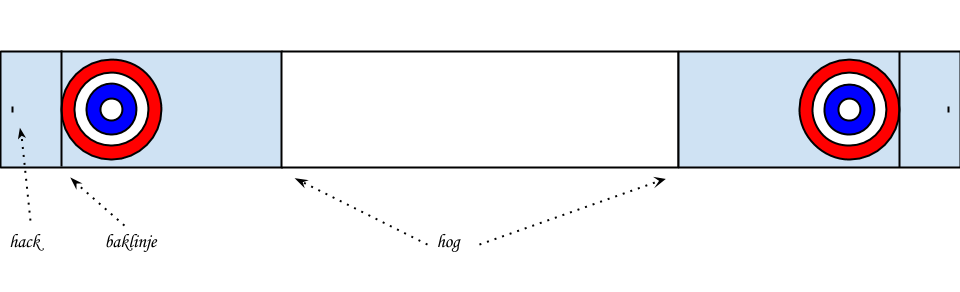
\includegraphics[width=110mm]{bana.png}
\caption{Curlingbanan}
\label{fig:bana}
\label{overflow}
\end{figure}


\begin{align}%\label{vtot}
 \omega_0 = \frac{\pi}{2 t_0} 
 \end{align}


Friktionen som påverkar rotationshastigheten är summan av all friktion som påverkar bandet som stenen roterar på. Detta kan sammanfattas till friktionen i de två punkterna, p1 och p2 på stenen. Accelerationen på stenens rotation kan därmed beräknas som accelerationen i de två punkterna. 

 \begin{align}\label{a_rotation1}
 \alpha_{rot} =- \frac{( a_1 + a_2)}{r} = -\frac{(\mu_1 g + \mu_2 g)}{r} = - g\frac{c_1+c_2}{r \sqrt{v_f}}
 \end{align}
 

\subsection{Kollision}

För att kontrollera att en kollision sker beräknas avståndet mellan stenarnas position \eqref{d}.
Om avståndet mellan stenarnas mittpunkter är mindre än två radier \eqref{lessThan} har stenarna krockat  (eftersom krocken bara sker i 2 dimensioner). 

 \begin{subequations}\label{d}
 \begin{align}
 d& = \sqrt{(sten_{1_{xpos}} - sten_{2_{xpos}})^2   +   (sten_{1_{ypos}}-sten_{2_{ypos}})^2}\\\label{lessThan}
 d& \le 2 r
 \end{align}
 \end{subequations}

\begin{figure}[ht!]
\centering
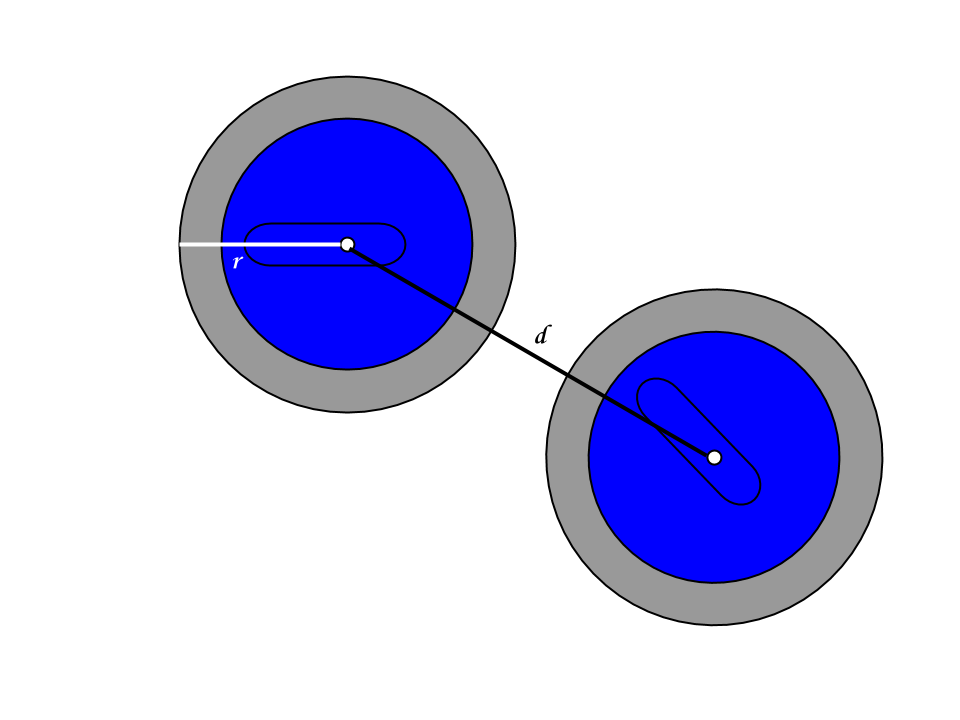
\includegraphics[width=80mm]{krock.png}
\caption{Kontrollera kollision}
\label{fig:kollision}
\label{overflow}
\end{figure}
Hastigheten av curlingstenarna efter en kollision beräknas med hjälp av de två stenarnas position och hastighetsvektorer.
Beräkningarna utgår ifrån en rak central stöt i krockens normalriktning, där det finns två givna ekvationer \eqref{e1} och \eqref{elastisk} för att ta fram hastigheten efter krock. 
Med hjälp av stötkoefficienten e \eqref{e1} kan stöten regleras mellan en helt elastikt krock (e=1) och en helt inelastiskt krock (e=0). 
I curling är det rimligt med en energiförlust och en inelastisk stöt bör därmed tas i beräkning. 
Stötkoefficienten är kvoten av den relativa hastigheten efter kollision och den relativa hastigheten före kollision enligt \eqref{e1}.

Eftersom det ej finns en specificerad stötkoefficient för curlingstenarnas material (granit) har en stötkoefficient uppskattats till 0.3 genom simuleringar.  

 \begin{subequations}\label{e1}
 \begin{align}
 e& = \frac{v_2''-v_1''}{v_2'-v_1'}\\
0& \le e \le 1
 \end{align}
 \end{subequations}

REFERENS: R Grahn,P-Å jansson: Dynamik (Studentlitteratur 1995), sid 334-345
\\\\Oavsett om krocken är inelastisk eller elastisk, gäller lagen om rörelsemängdens bevarande.

 \begin{subequations}\label{elastisk}
 \begin{align}
m_1 v_1' + m_2 v_2'& = m_1 v_1'' + m_2 v_2'' \Rightarrow\\
m_1& = m_2 \Rightarrow\\
v_1' + v_2'& = v_1'' + v_2'' \label{momentum}
 \end{align}
 \end{subequations}

\pagebreak

Hastigheterna delas upp i en normal- och tangentkomponent genom att projicera hastighetsvektorn på krocknormalen \eqref{e_normal} och tangentnormalen. Hastighetsvektorn delas upp i dessa komponenter eftersom energiförlusten enbart sker i normalkomponentens riktning. Genom att addera tangentkomponenten med normalkomponenten efter energiförlust, kan sneda krockar hanteras.

 \begin{align}\label{e_normal}
e_n& = \overrightarrow{OP_2} -  \overrightarrow{OP_1}  
 \end{align}

Där $P_1$ och $P_2$ är stenarnas position. Tangentnormalen är ortogonal mot krocknormalen. $e_n$ ses i Figur~\ref{fig:kollision-vektorer}. 

 \begin{align}\label{vCollision}
v_1'& = v_{1n}' + v_{1t}'\\
v_2'& = v_{2n}' + v_{2t}'
 \end{align}

\begin{figure}[ht!]
\centering
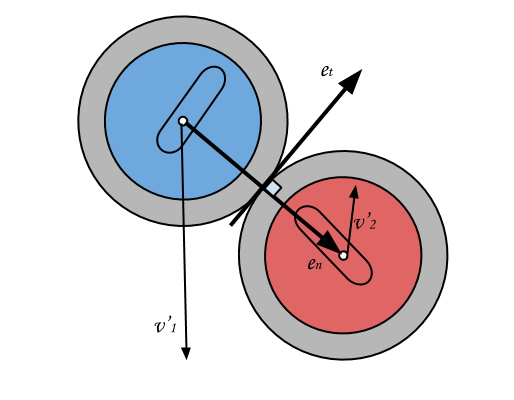
\includegraphics[width=69mm]{kollision-vektorer.png}
\caption{Kollision med riktningar för hastigheter innan krock där $v_{1}$ har högre fart än $v_{2}$}.
\label{fig:kollision-vektorer}
\label{overflow}
\end{figure}

Kollisionen räknas ut som en rak central stöt med normalkomponenterna, $v_{1n}'$ och  $v_{2n}'$ insatta i ekvation \eqref{e1} och \eqref{momentum}. Hastigheterna efter krocken löses sedan ut, \eqref{vCollision2} och \eqref{vCollision2n}.

 \begin{align}\label{vCollision2}
 v_{1n}''& = \frac{v_{1n}' + v_{2n}'  - e(v_{1n}' + v_{2n}')}{2} \\
 v_{2n}''& = \frac{v_{1n}' + v_{2n}'  + e(v_{1n}' + v_{2n}')}{2} \label{vCollision2n}
 \end{align}

\pagebreak

För att få den resulterande hastigheten adderas normalkomponenten efter krock med tangentkomponenten. Illustration hittas i Figur~\ref{fig:efter-krock}. 
 \begin{align}\label{vfinal}
v_1''& = v_{1n}'' + v_{1t}'\\
v_2''& = v_{2n}'' + v_{2t}'
 \end{align}

\begin{figure}[ht!]
\centering
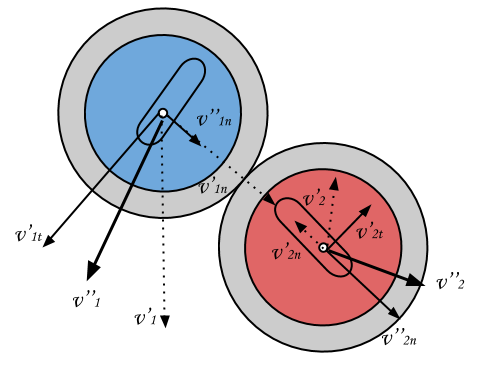
\includegraphics[width=90mm]{efter-krock.png}
\caption{Efter en kollision med normalkomponenterna för hastigheten innan och efter och även den slutgiltiga hastigheten.  }.
\label{fig:efter-krock}
\label{overflow}
\end{figure}


\section{Numerisk}
Tre farter beräknas i varje steg av simuleringen: fart i rörelseriktningen, fart i ortogonal riktning som tillför curl samt vinkelhastighet. Dessa beräknas genom Runge-Kutta-metoden enligt \eqref{RungeKutta_transl}. 

 \begin{subequations}\label{RungeKutta_transl}
 \begin{align}
 v_{n+1}& =v_n + \frac{h}{6} (k_1+2 k_2 + 2 k_3 + k_4)\\
 k_1& = a(v_n)\\
 k_2& = a(v_n + \frac{h}{2} k_1)\\
 k_3& = a(v_n + \frac{h}{2} k_2)\\
 k_4& = a(v_n + h k_3)
 \end{align}
\end{subequations}

Funktionen a för accelerationen för de olika farterna olika beroende på de olika friktionstillstånden enligt \eqref{a_front},  \eqref{a_side}, \eqref{a_rotation}.
 
 \begin{align}\label{a_front}
 a_{fram}& = - \mu g\\\label{a_side}
 a_{sida}& = g \frac{c_2-c_1}{\sqrt{v_f}}\\\label{a_rotation}
 a_{rot}& = \alpha_{rot} = - g\frac{c_1+c_2}{r \sqrt{v_f}}
 \end{align}

Samtliga tre parametrar (fart framåt, fart i sidled och vinkelhastighet) är skalärer. Efter att nästa värde erhållits genom Runge-Kutta-metoden tas hastigheten i riktning framåt och i sidled fram och de två adderas genom vektoraddition. Ny position av stenen beräknas i sista steget genom Euler-metoden, där hastighetsvektorn anger riktning och steglängd \eqref{pos}. 

 \begin{align}\label{pos}
 pos_{n+1}& = pos_{n} + \bar{v} \Delta t
 \end{align}


\section{Grafisk implementering}
Blender, webGL, blablabla

\pagebreak
\section{Resultat}

Lite grejer från matlab osv. 
Lagt in lite diverse grafer.
Rada upp alla konstanter som används i simuleringen. 

\begin{figure}[ht!]
\centering
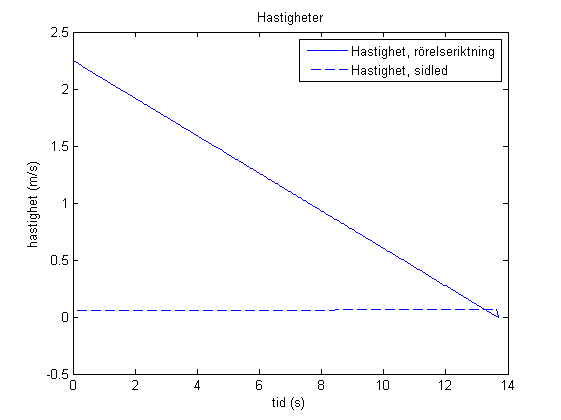
\includegraphics[width=100mm]{hastigheter_tid_graf.png}
\caption{Hastigheter i färdriktning och i sidled som funktion av tid.}
\label{fig:hast_graf}
\label{overflow}
\end{figure}

\begin{figure}[ht!]
\centering
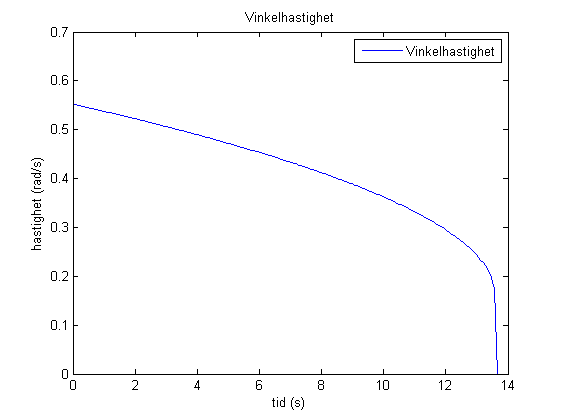
\includegraphics[width=100mm]{vinkelhastighet_tid_graf.png}
\caption{Vinkelhastighet som funktion av tid.}
\label{fig:vinkelhast_graf}
\label{overflow}
\end{figure}


\section{Diskussion}


\appendix
\section{\\Title of Appendix A} \label{App:AppendixA}
Kanske lägga in alla benämningar av konstanter osv.

\end{document}
